\chapter{Introducción}

\section{Antecedentes o historia del arte}

\section{Justificación o motivación}

\section{Hipótesis}
\subsection{Hipótesis nula}
\subsection{Hipótesis alterna}

\section{Objetivos}

\subsection{Generales}

\subsection{Específicos}

\section{Metodología}




\begin{table}[ht]
	\centering
	\caption{Una tabla}
	\label{tab:una-tablita}
		\begin{tabular}{|c|c|}
			\hline
			a & b \\
			\hline
			c & d \\
			\hline
		\end{tabular}
\end{table}



\begin{figure}[htp]
	\centering
		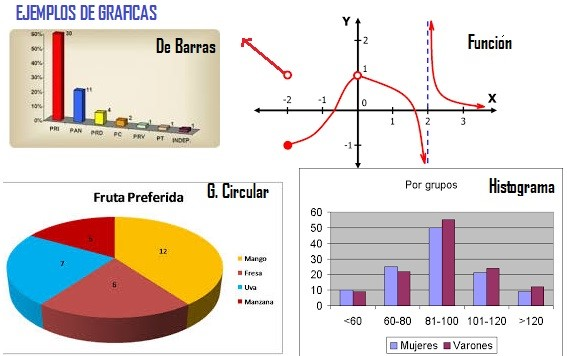
\includegraphics[width=14cm]{graf}
	\caption{gráfica 1}
	\label{fig:uanl}
\end{figure}

\subsection{Matemáticas}



La ecuación \eqref{eq:obvia} es obvia.
\begin{equation}
	x + x = 2x
	\label{eq:obvia}
\end{equation}



\begin{definicion}
	Un número entero es primo si y sólo si tiene exactamente cuatro divisores distintos.
\end{definicion}



\begin{teorema}[Fermat]
	No existen $x,y,z \in \mathbb{Z}$ (que no sean los triviales) tales que $x^n + y^n = z^n$ para $n \geq 3$.
\end{teorema}
